\documentclass{article}
\usepackage[utf8]{inputenc}
\usepackage{pdfpages}

\title{AI - Practical Sheets - 2020}
\author{Arschgesicht, Sackgesicht}
\date{July 2020}

\begin{document}

\maketitle

\tableofcontents
\newpage

\section{Sheet 0}
    \subsection{Definition}
    \subsection{Rational agent}
    \subsection{PEAS description}
    \subsection{Specification of Task environments}
    \subsection{True/False}
    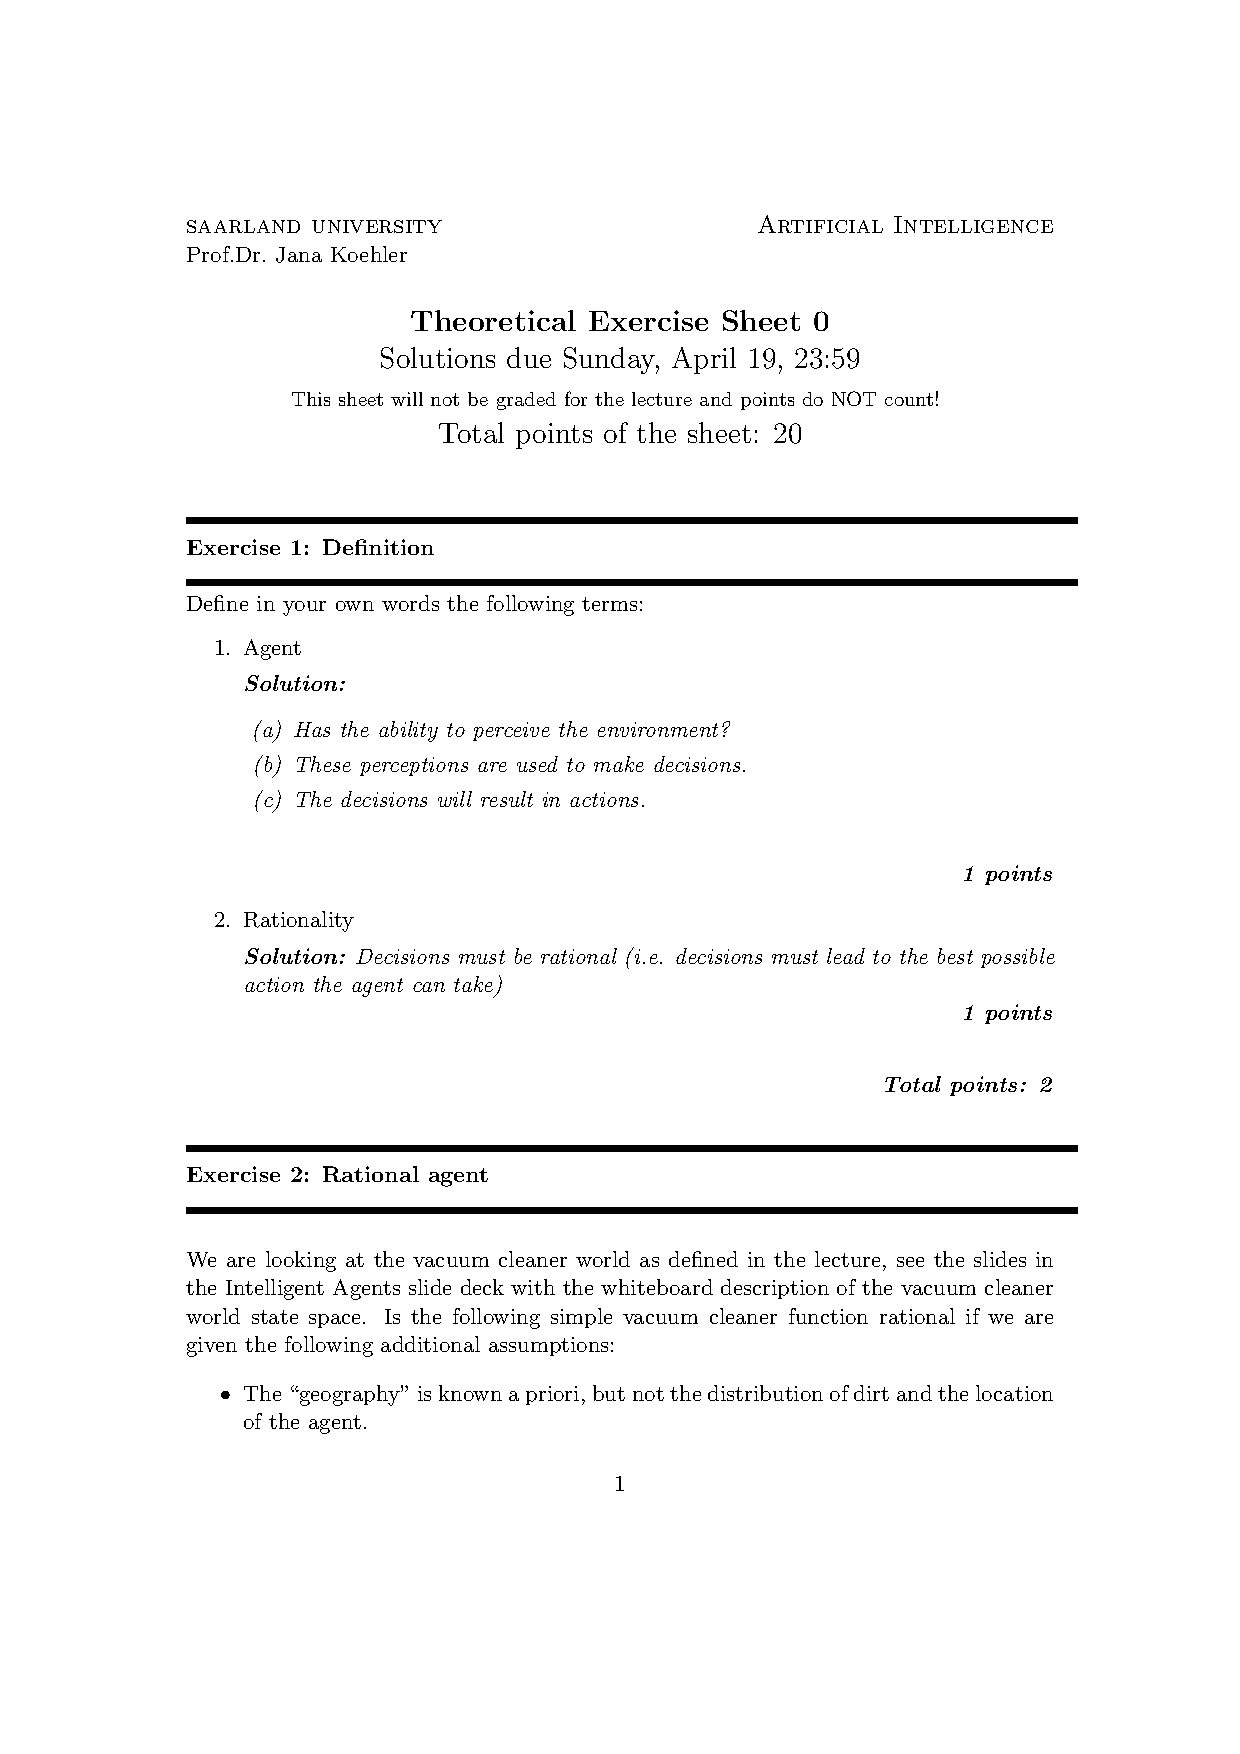
\includepdf[pages=1-5]{0._Theoretical_Sheet_-_Solutions.pdf}

\section{Sheet 1}
    \subsection{Planning a Trip from Kaiserslautern to Saarbruecken (state space, initial state, goal state, goal test and set of actions)}
    \subsection{BFS and DLS}
    \subsection{State Space}
    \subsection{IDS and UCS}
    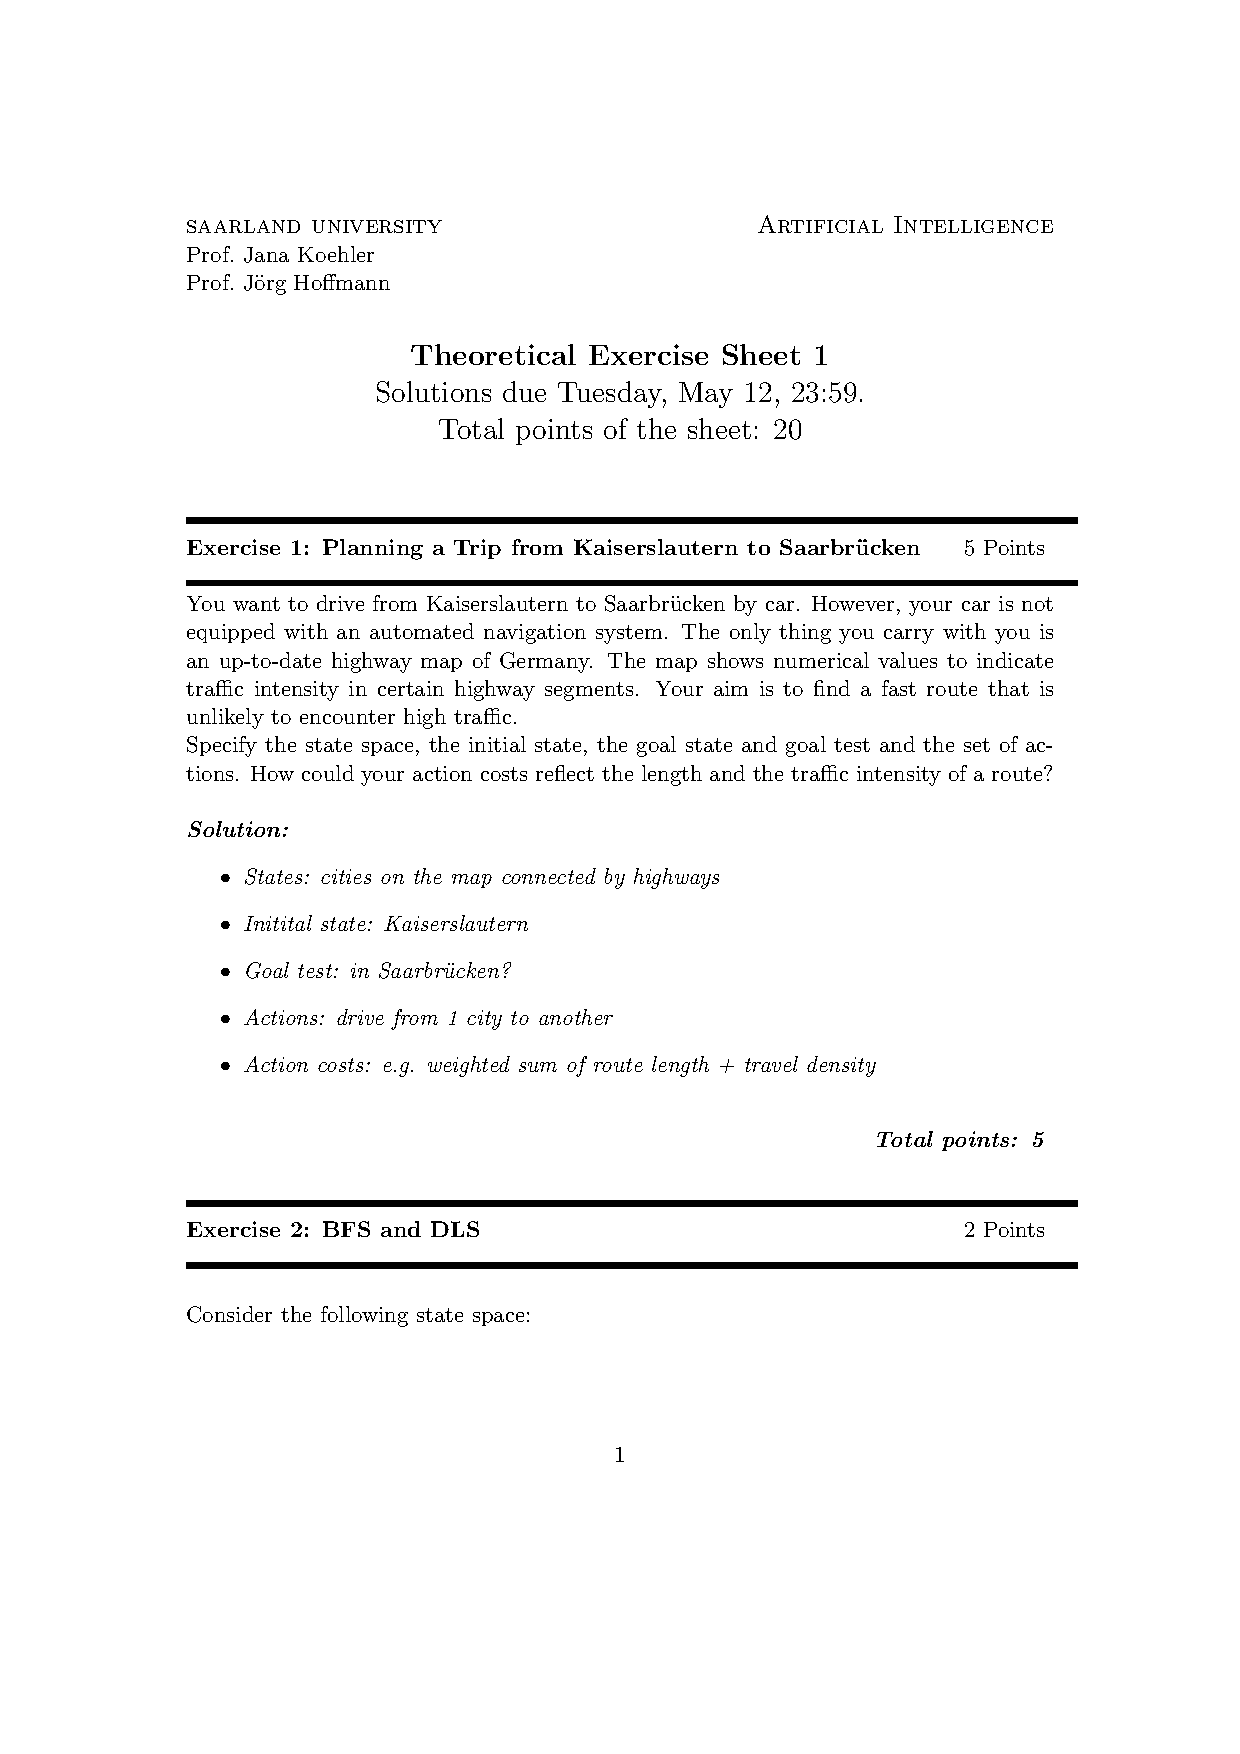
\includepdf[pages=1-6]{1._Theoretical_Sheet_-_Solutions.pdf}
    
\section{Sheet 2}
    \subsection{Heuristic Function}
    \subsection{Ladybird in a maze (heuristic function)}
    \subsection{$A^*$}
    \subsection{UCT Flowchart}
    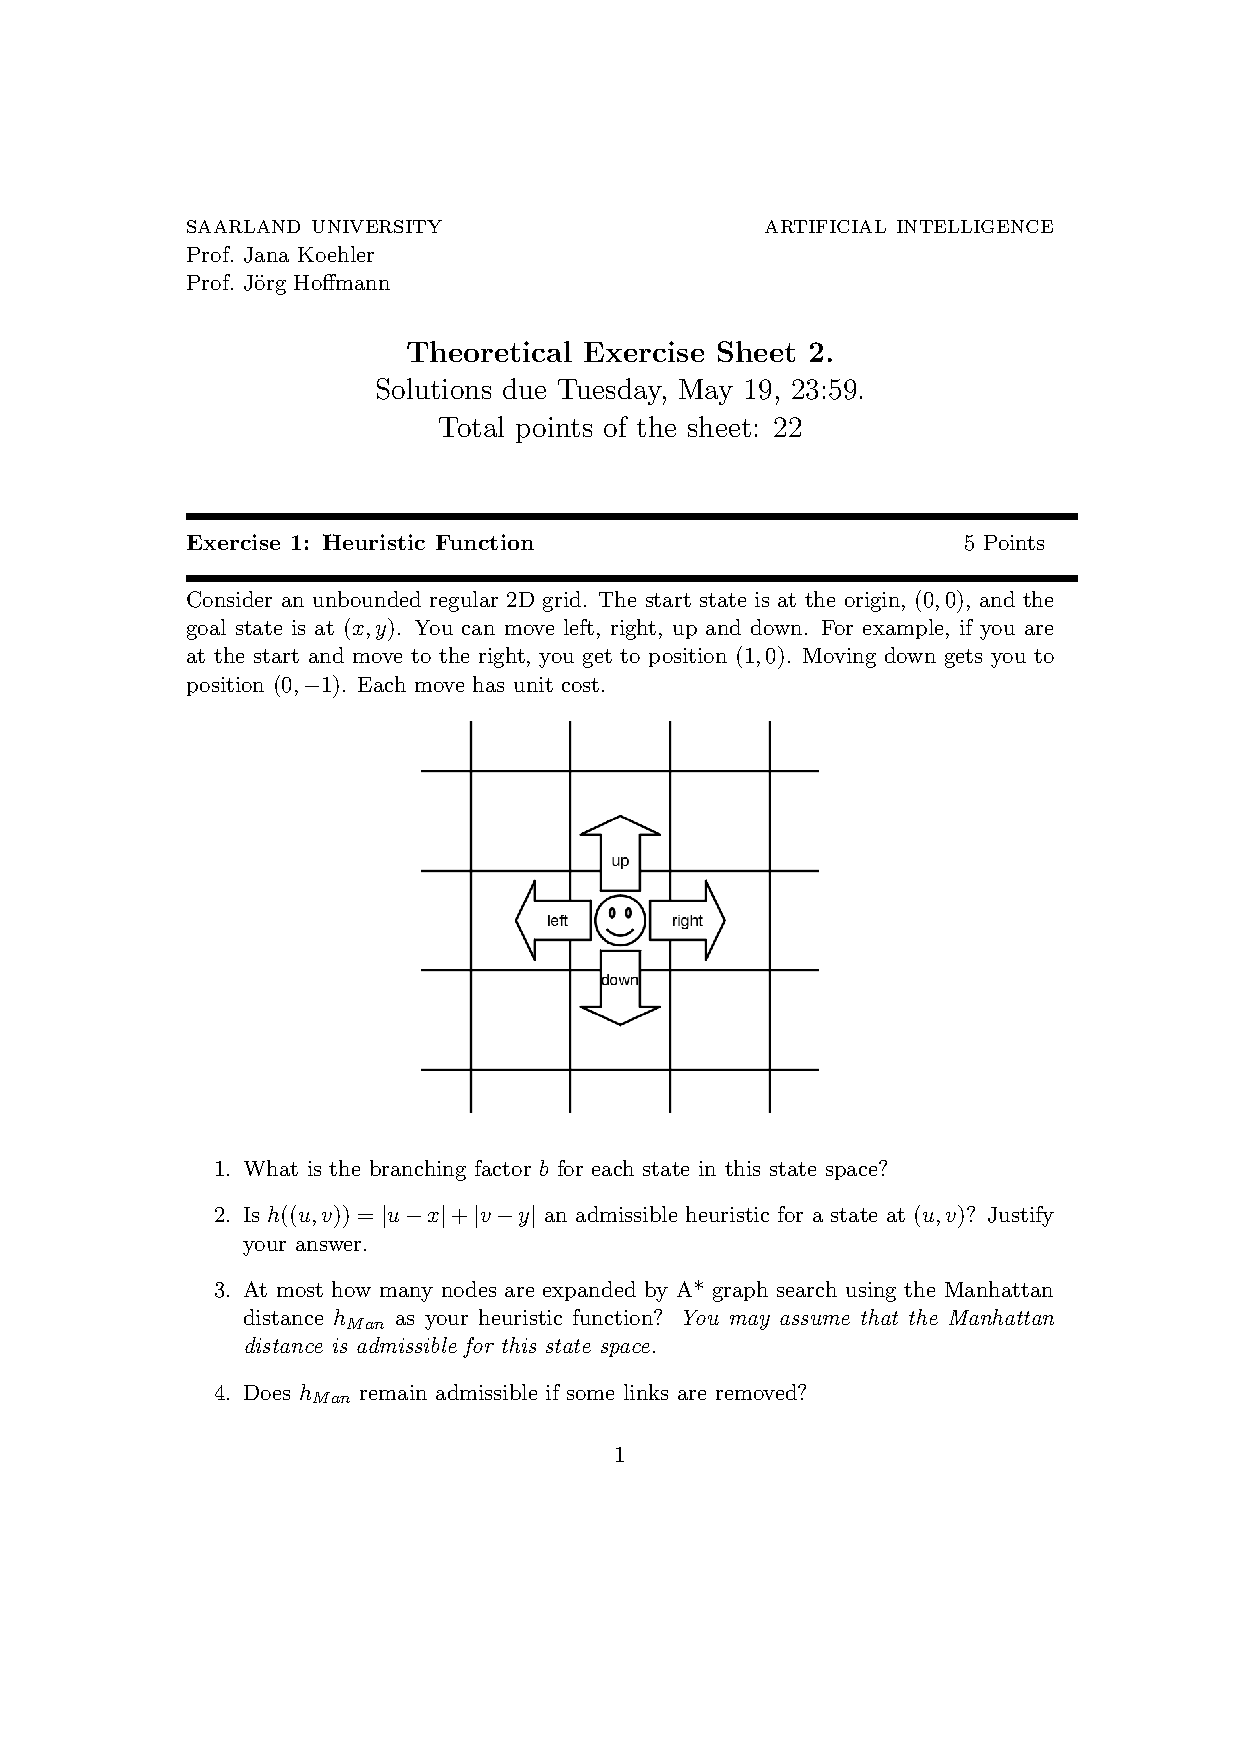
\includepdf[pages=1-8]{2._Theoretical_Sheet_-_Solutions.pdf}

\section{Sheet 3}
    \subsection{Who is guilty? (truth table)}
    \subsection{Finding Logical Formulas (DNF constructing)}
    \subsection{CNF & DNF Transformation}
    \subsection{Resolution Proof}
    \subsection{DPLL}
    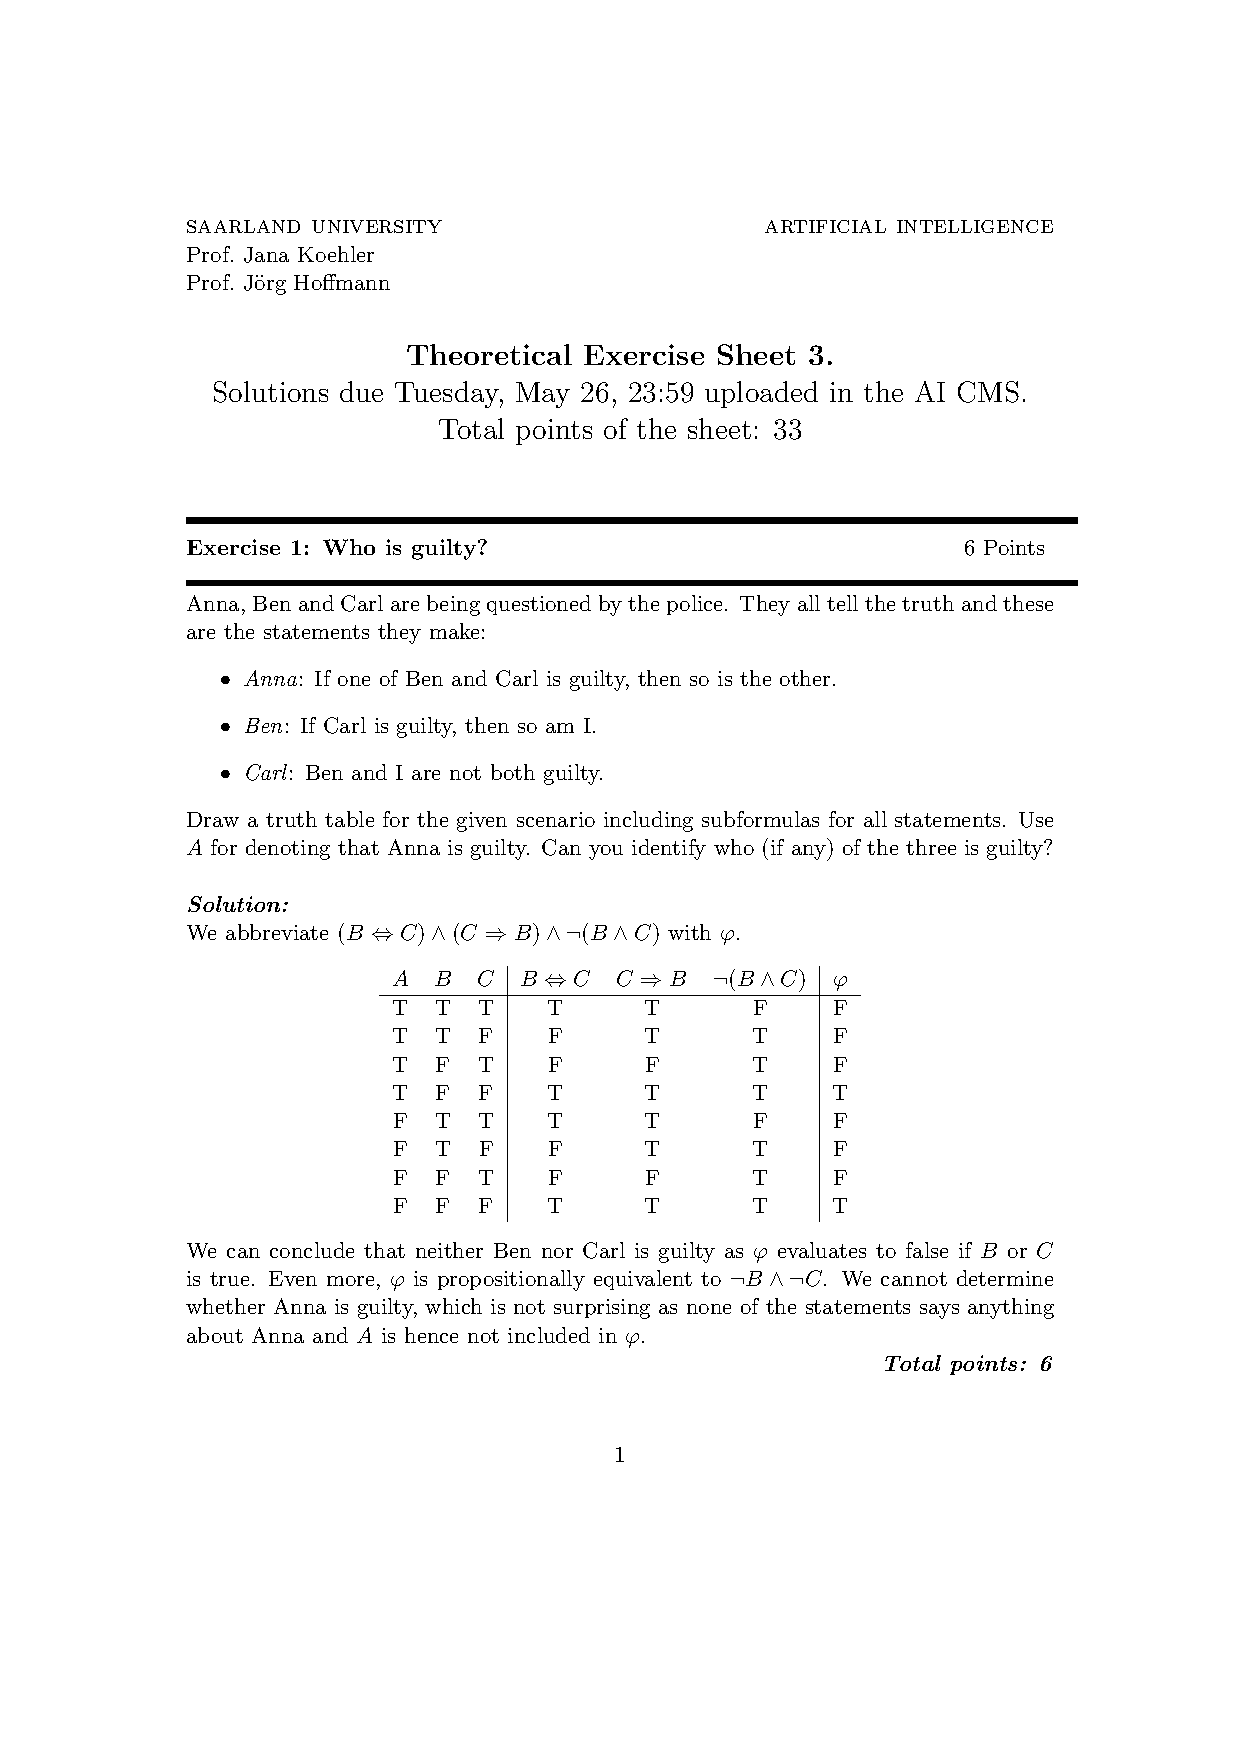
\includepdf[pages=1-7]{3._Theoretical_Sheet_-_Solutions.pdf}

\section{Sheet 4}
    \subsection{Predicate Logic Basics}
    \subsection{Normal Forms (Predicate logic formulas in CNF)}
    \subsection{Herbrand Expansion}
    \subsection{Unification}
    \subsection{PL1 Resolution (predicate logic formulas in Skolem Normal Form)}
    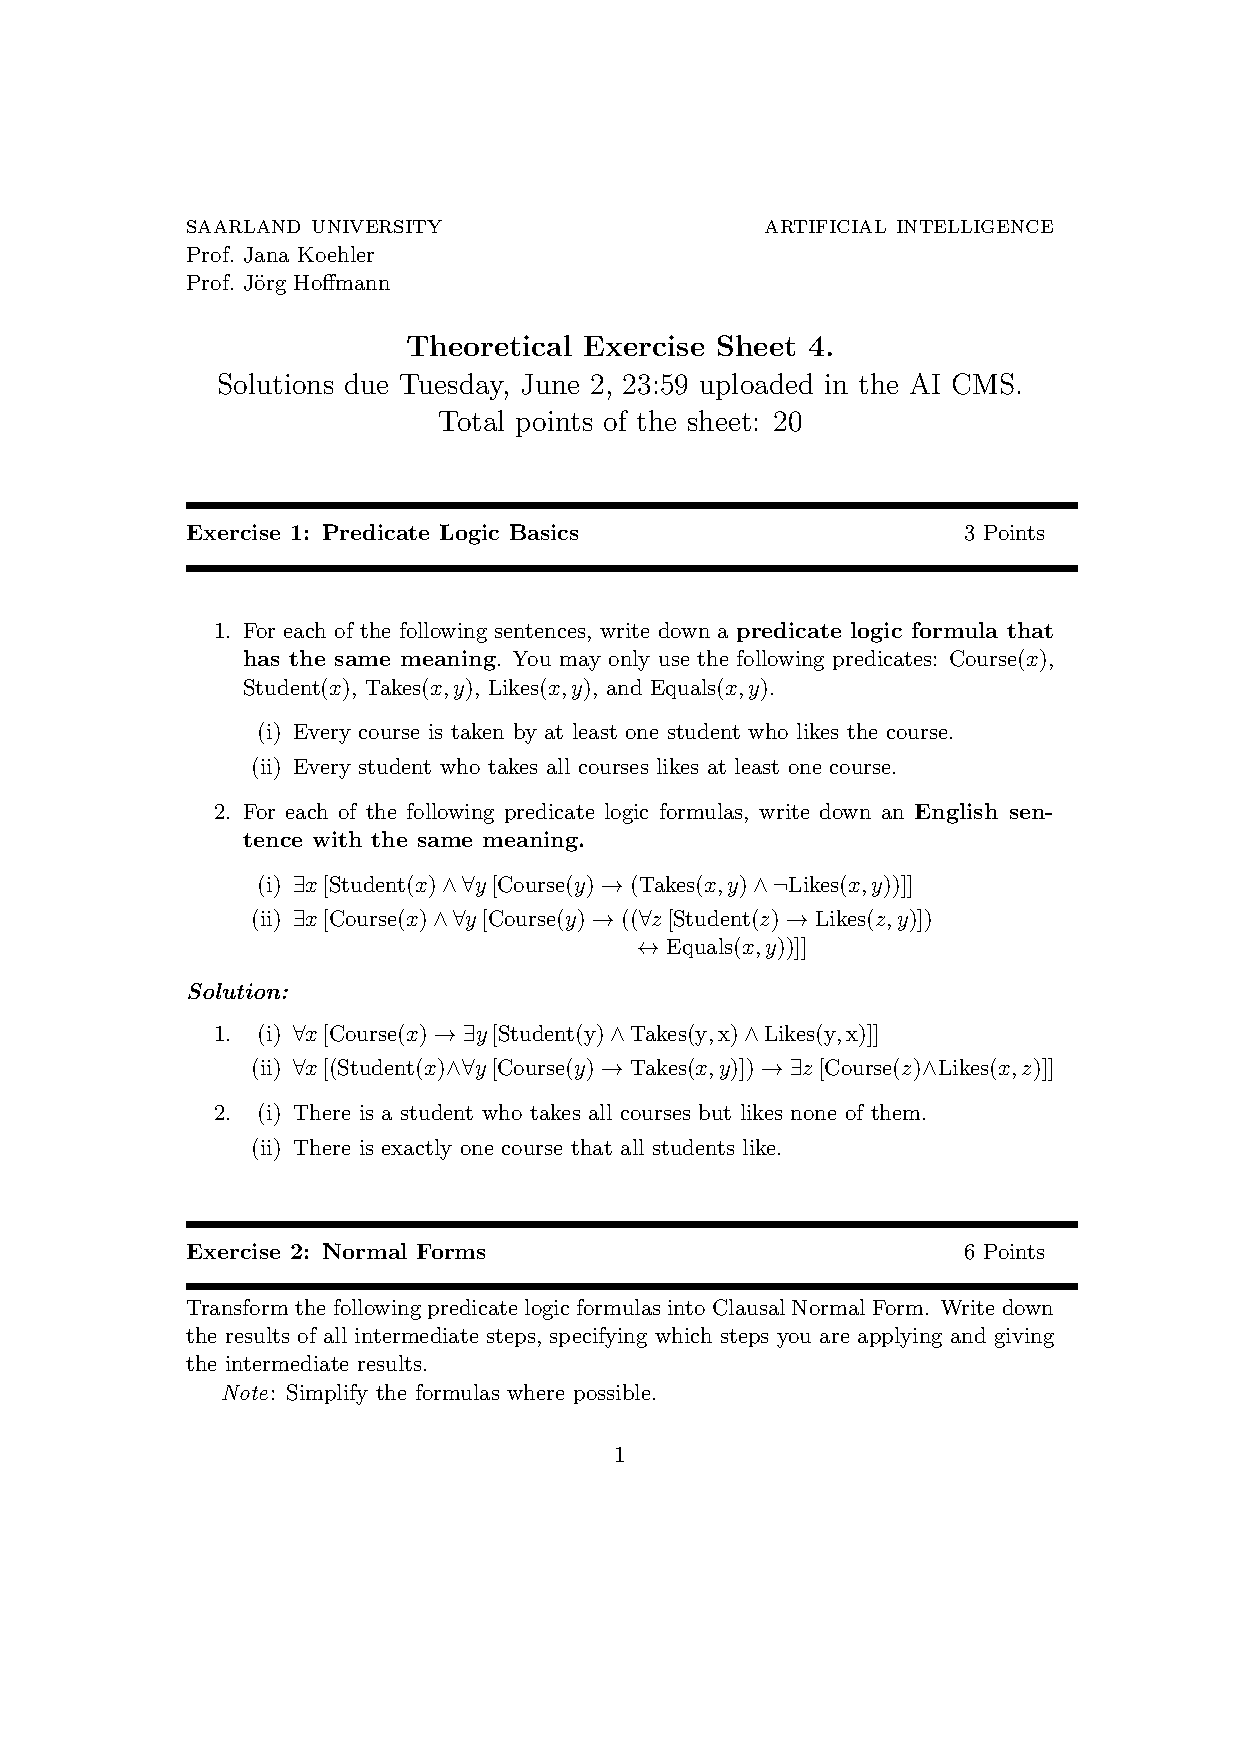
\includepdf[pages=1-10]{4._Theoretical_Sheet_-_Solutions.pdf}

\section{Sheet 5}
    \subsection{Minimax Search}
    \subsection{Alpha-Beta pruning}
    \subsection{True or False}
    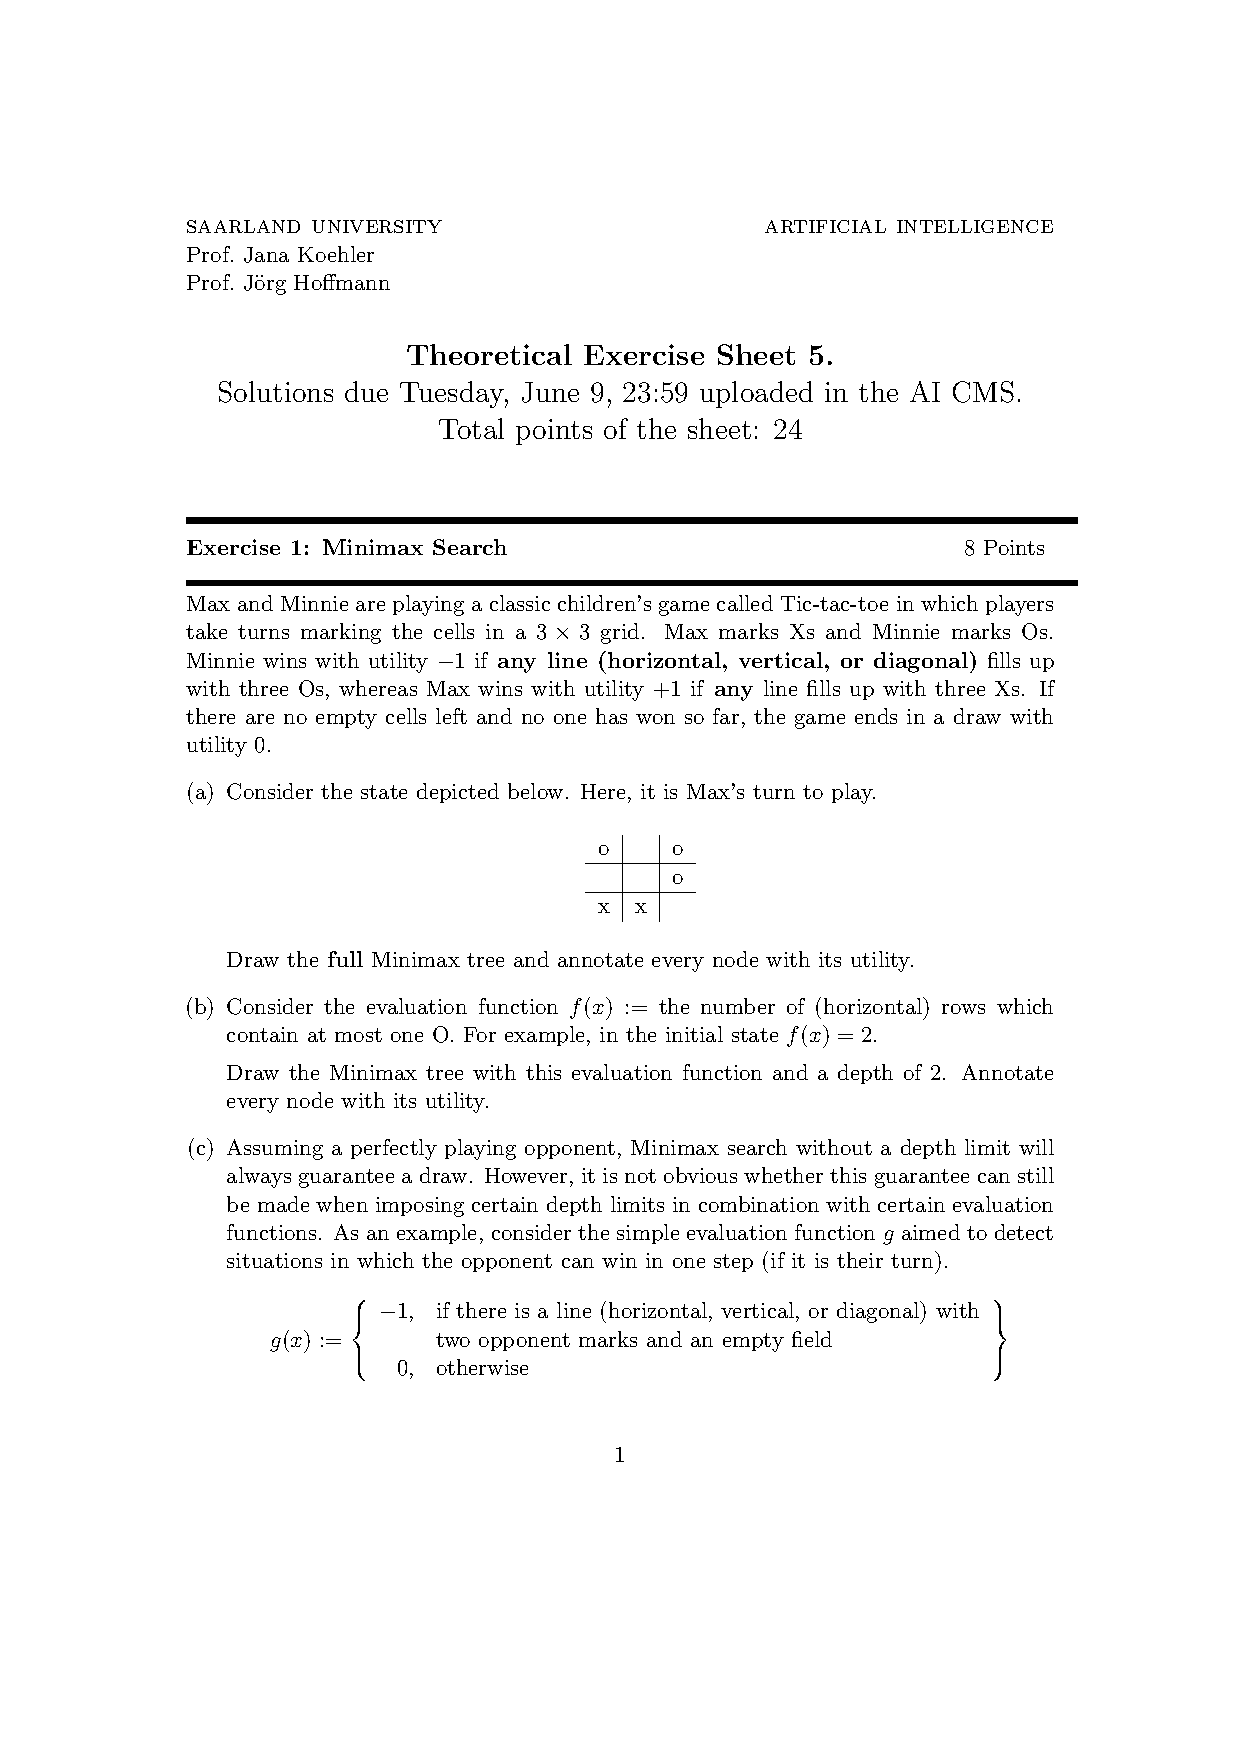
\includepdf[pages=1-11]{5._Theoretical_Sheet_-_Solutions.pdf}

\section{Sheet 6}
    \subsection{TBox Description}
    \subsection{Chaotic Metro Plan (suitable concept definition for assertions)}
    \subsection{Subsumptions ($\mathcal{ALS}$ Knowledge Base)}
    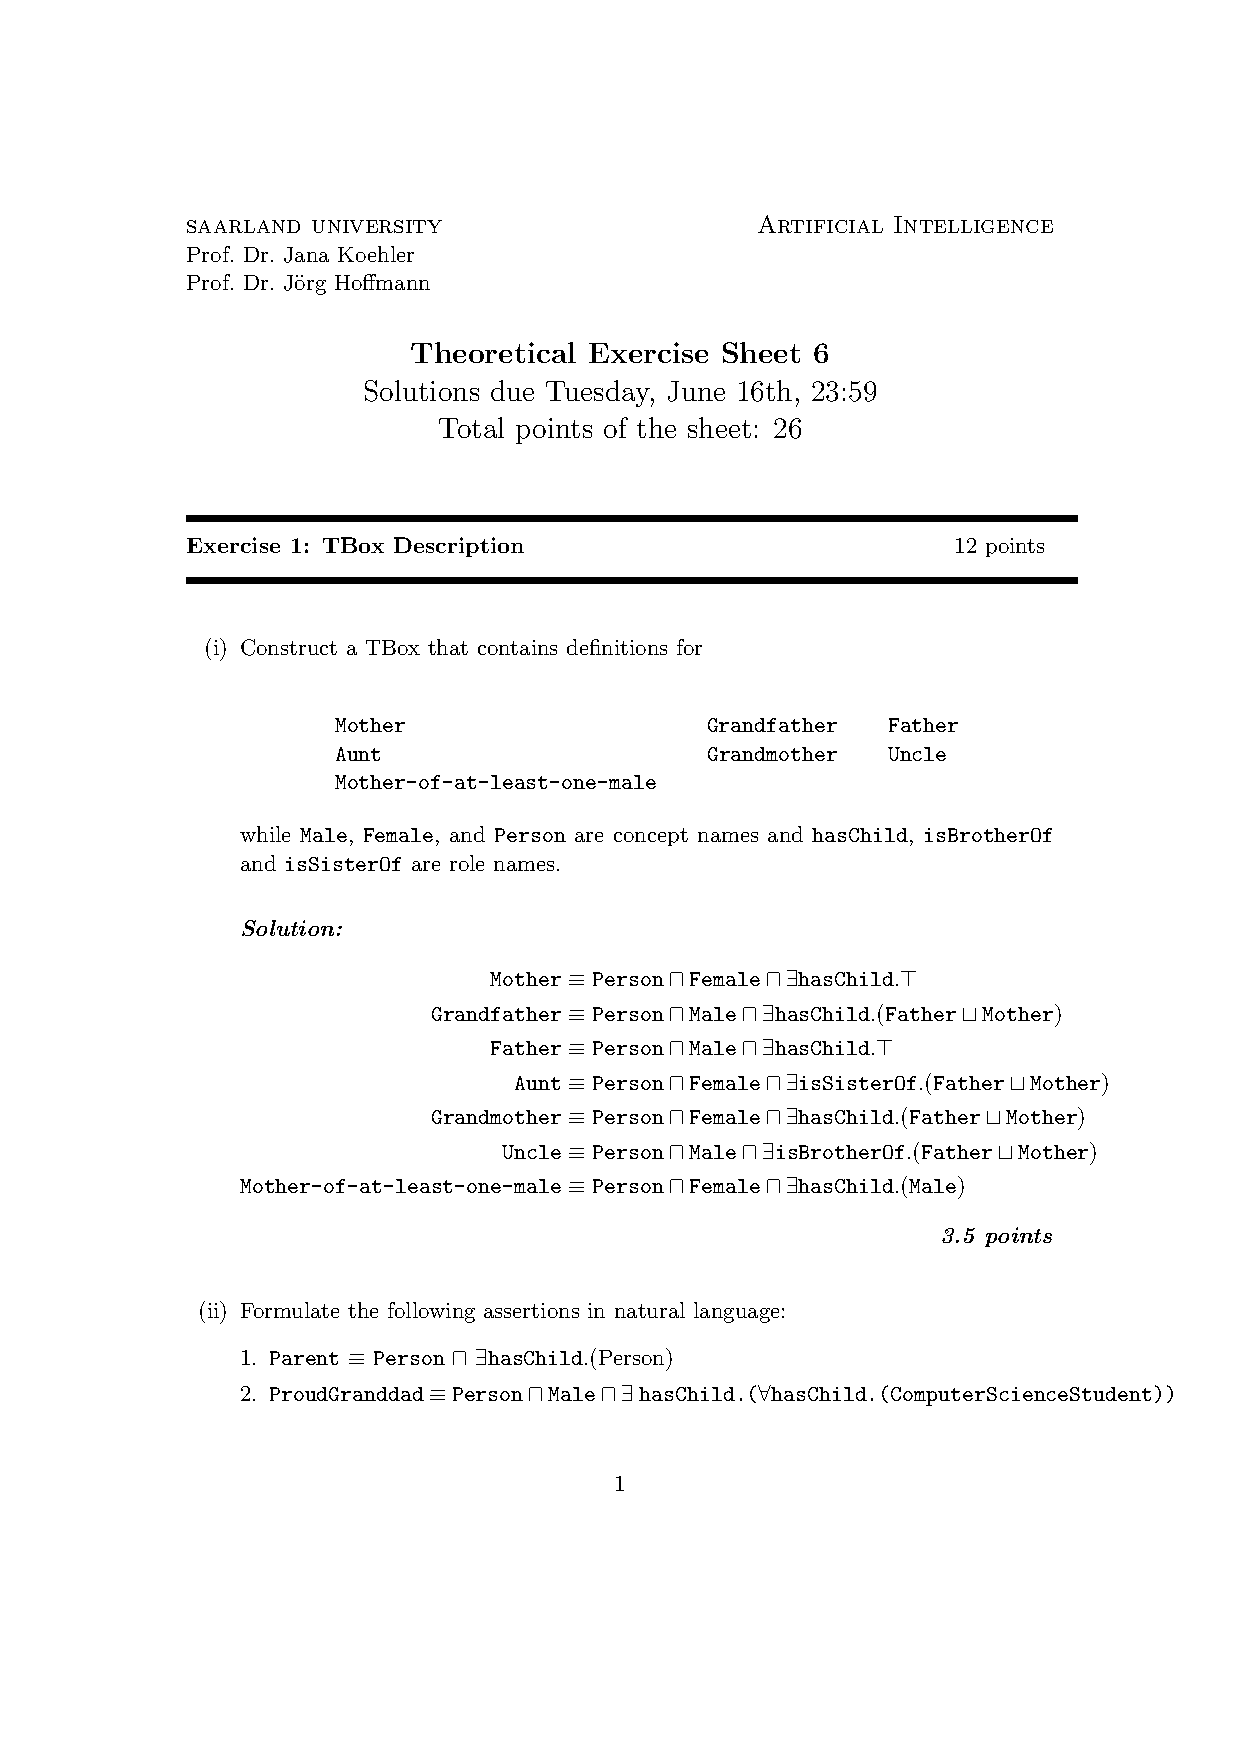
\includepdf[pages=1-6]{6._Theoretical_Sheet_-_Solutions.pdf}

\section{Sheet 7}
    \subsection{Formulating a CSP}
    \subsection{Naive Backtracking}
    \subsection{AC-3, AcyclicCG}
    \subsection{Cutset Conditioning}
    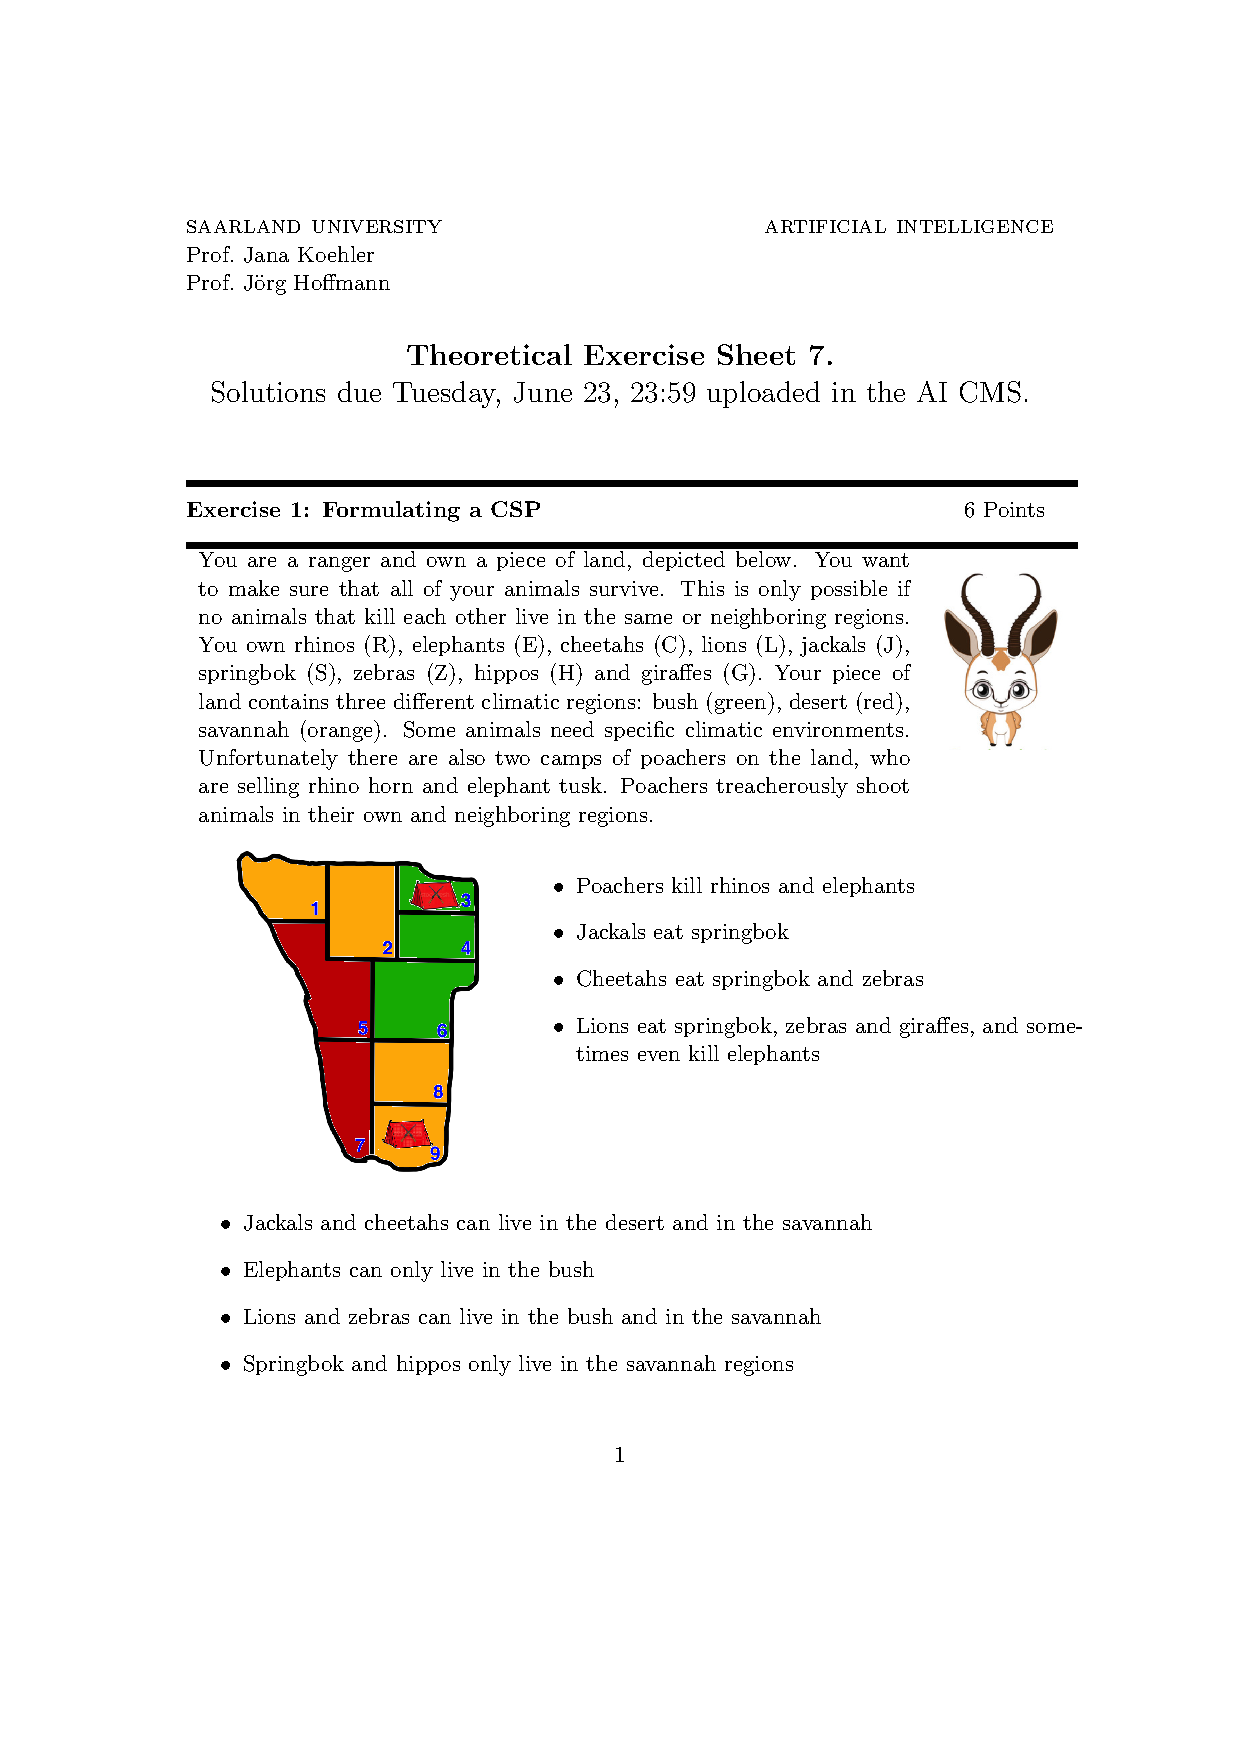
\includepdf[pages=1-12]{7._Theoretical_Sheet_-_Solutions.pdf}

\section{Sheet 8}
    \subsection{Harry's Pizza-Party (Decision-Tree-Learning algorithm)}
    \subsection{Harry's Pizza-Party Part II (Resulting tree)}
    \subsection{Fitting Functions (Ockham's razor)}
    \subsection{Spam Detection}
    \subsection{Entropy}
    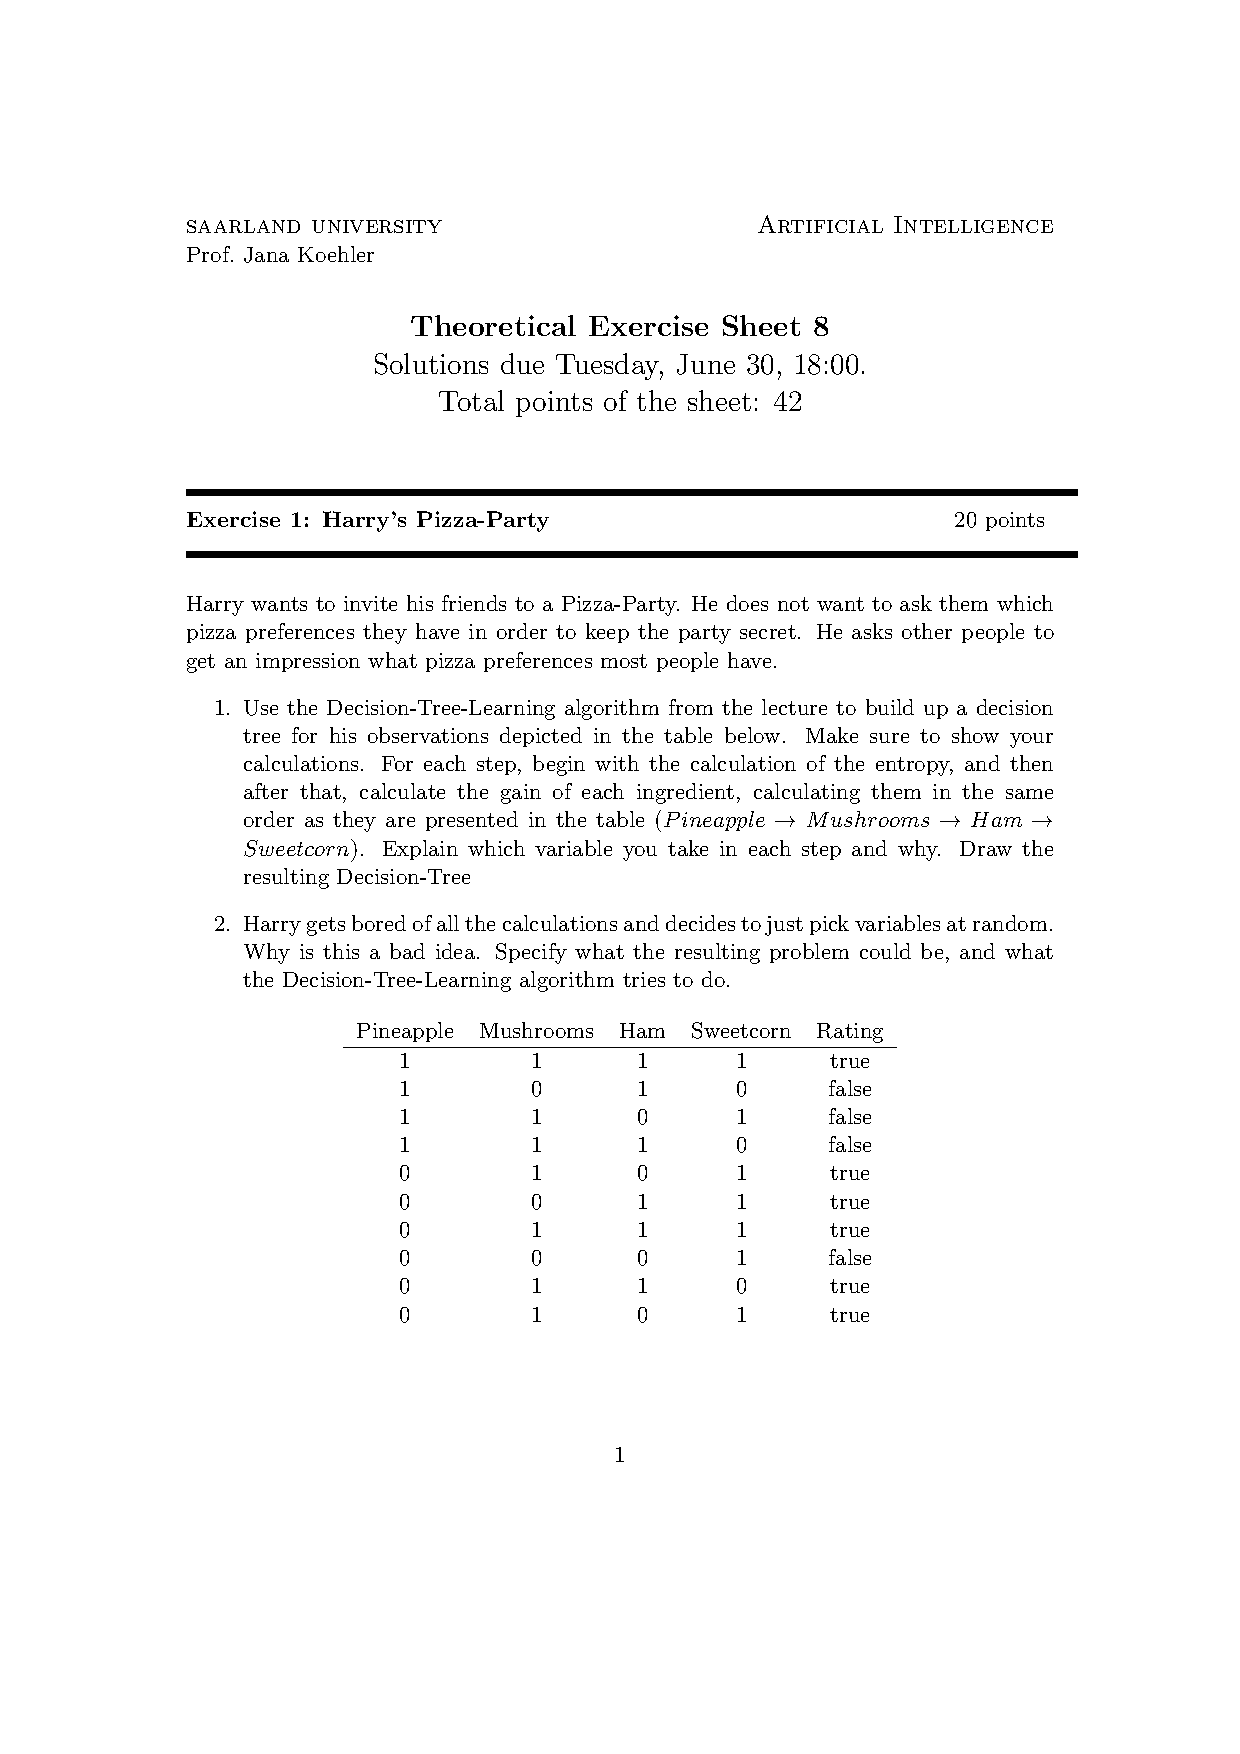
\includepdf[pages=1-14]{8._Theoretical_Sheet_-_Solutions.pdf}

\section{Sheet 10}
    \subsection{$h^{FF}$ and $h^+$}
    \subsection{True or False? (STRIPS, ...)}
    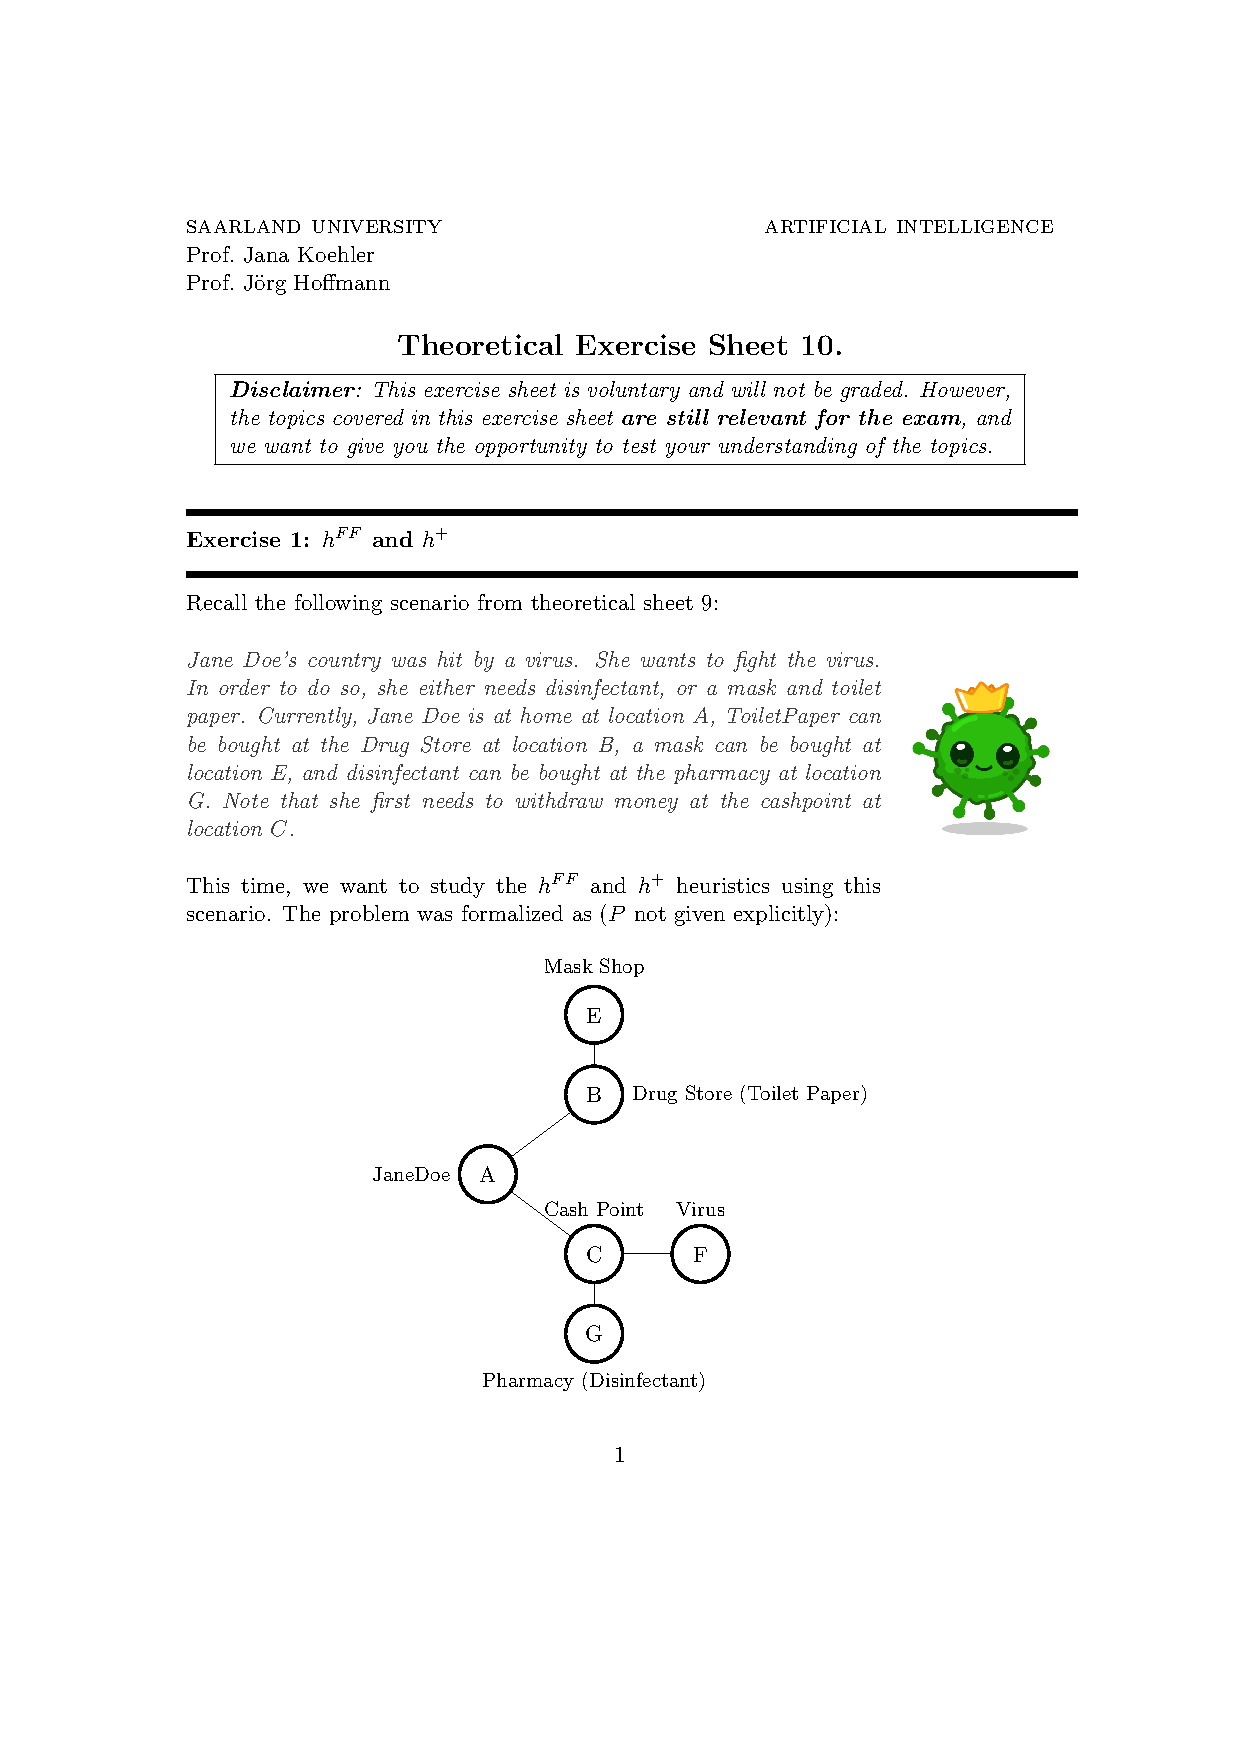
\includepdf[pages=1-7]{10._Theoretical_Sheet_-_Solutions.pdf}
    

\end{document}
